\documentclass{report}

%Character encoding
\usepackage[utf8]{inputenc}
\usepackage[T1]{fontenc}
%The language
\usepackage[french]{babel}

%Including pictures
\usepackage{graphicx}
\usepackage{rotating}

%The page lookout
\usepackage[margin=2cm]{geometry}
\usepackage{fancyhdr}
\pagestyle{fancy}
\lhead{PLD-COMP - Rapport de mi-parcours\\The super 4404 Compiler}
\rhead{H44(0/1)4 - A. Belin, A. Nahid, L. Ohl, L. Saos, A. Verrier, I. Zemmouri}
\cfoot{\thepage}

%Make references
\usepackage{hyperref}
\usepackage{url}

%Math symbols
\usepackage{amssymb}

%Quoting code
\usepackage{listings}
\usepackage{color}
\lstdefinestyle{cpp}{
	backgroundcolor=\color{white},
	basicstyle=\footnotesize,
	breakatwhitespace=false,
	breaklines=true,
	commentstyle=\color{green},
	frame=single,
	keywordstyle=\color{blue},
	numbers=left,
	numbersep=5pt,
	numberstyle=\tiny,
	showspaces=false,
	stringstyle=\color{red},
	tabsize=2,
	language=C++
}

\lstdefinestyle{make}{
	backgroundcolor=\color{white},
	basicstyle=\footnotesize,
	breakatwhitespace=false,
	breaklines=true,
	commentstyle=\color{black},
	frame=single,
	keywordstyle=\color{green},
	showspaces=false,
	stringstyle=\color{yellow},
	tabsize=2,
	language=make
}
\lstset{style=cpp}

%Removing the chapter number in sectionning
\makeatletter
\renewcommand{\thesection}{\@arabic\c@section}
\makeatother

\title{PLD-COMP\\Rapport de mi-parcours}
\author{H4414\\A. Belin - A. Nahid - L. Ohl\\L. Saos - A. Verrier - I. Zemmouri}

\begin{document}
\maketitle
\tableofcontents
\section*{Un petit mot d'introduction}

Ce dossier reprend l'ensemble des points produits et demandés pour le Projet Longue Durée Compilateur, à savoir compiler n très simple programme C consistant d'un main et d'affectation arithmétiques sur des entiers.\\
Toutefois, qui dit mi-parcours dit aussi \og en cours de route \fg. Il ne sera donc pas étonnant de trouver des aspects grammaticaux, sémantiques, etc, développés en avance par rapport au travail demandé. Ces points particuliers seront décrits en annexes, car n'étant pas au coeur du sujet.

\section{Fonctionalités implémentées}
\label{sec:Fonc}

Nous allons survoler dans cette section l'ensemble des possibles actuellements réalisable par notre compilateur.

\subsection{Ce que le front peut lire}
\label{subsec:Front}

Par \og ce que le front peut lire \fg, nous entendons ce que le parser est capable de lire et, en addition, transformer sa lecture en éléments de l'ast. Autrement dit, ce n'est pas que de la grammaire !\\

Le parser est capable de lire un corps de main contenant une série de définitions, suivi par l'ensemble des instructions arithmétiques et une éventuelle instruction return.

Voici des exemples de corps main tolérés\footnote{Pour tout ce qui suivra, les commentaires sont uniquement pour la compréhension de ce qui peut être écrit. En aucun cas le compilateur ne saura les lire. Ils doivent donc être absents des fichiers à compiler} :
\begin{lstlisting}
int main() {
	//...
}
\end{lstlisting}
\begin{lstlisting}
void main(){
	//...
	return;
}
\end{lstlisting}
\begin{lstlisting}
void main() {}
\end{lstlisting}
\begin{lstlisting}
int main() {
	//...
	return 23; //23 ou une expression arithmetique
}
\end{lstlisting}

Dans ce corps de main, il faut dans un premier temps déclarer et définir les variables qui seront utilisées dans le bloc de code.

\begin{lstlisting}
int a;
int a=3;
int a,b;
int a=2,b;
int a=3,b=4;
int c,d=a,e;
//idem avec char.
\end{lstlisting}

Enfin, les expressions arithmétiques suivantes sont opérables :
\begin{itemize}
\item L'addition +
\item La soustraction -
\item La multiplication *
\item La division /
\item Le \emph{et} bit-à-bit \&
\item Le \emph{ou} bit-à-bit $\|$
\item Le \emph{xor} bit-à-bit $\wedge$
\item L'opérateur unaire de négativation -
\item L'opérateur unaire \emph{not} $\thicksim$
\end{itemize}

Ainsi, le programme de mi-parcours est totalement lisible :
\begin{lstlisting}
int main()
{
int a,b,c;
a=17;
b=42;
c = a*a + b*b +1;
return c;
}
\end{lstlisting}

Bien sûr, il est encore tout à fait possible d'écrire n'importe quoi sémantiquement à ce stade-là. D'où la section suivante.

\subsection{La vérification sémantique}
\label{subsec:Seman}

Notre vérification sémantique du programme contient les éléments suivants pour le mi-parcours :

\paragraph{Pour le programme complet} Nous vérifions qu'il n'existe bien que des fonctions et des variables globales. Chacun sans duplicata. Nous vérifions également la présence de la fonction \emph{main}.\\

\paragraph{Pour une fonction} Nous vérifions récursivement la sémantique de chaque sous-instruction contenue. Nous vérifions également qu'elle ne possède pas de variables nommées similairement à d'autres variables de portée supérieure. Nous observons également si le \emph{return} d'une fonction corresond bien au type prétendu de la fonction.\\

\paragraph{Pour les expressions arithmétiques} Nous vérifions bien que les opérandes ne sont pas de type \emph{Void}, et vérifions que chaque sous-expression d'une expression est elle-même conforme. Enfin, pour ce qui est de l'affectation, nous vérifions systématiquement que l'identifiant d'une variable en l-value réfère bien quelque chose de connue et que la r-value est du même type que la l-value.\\

\subsection{Ce que le back peut écrire}
\label{subsec:Back}

\section{Structure du compilateur}
\label{sec:Struct}

\subsection{Répartition des packages}
\label{subsec:Pack}

Pour synthétiser l'ensemble : un petit schéma.

\begin{figure}[!hbt]\begin{center}
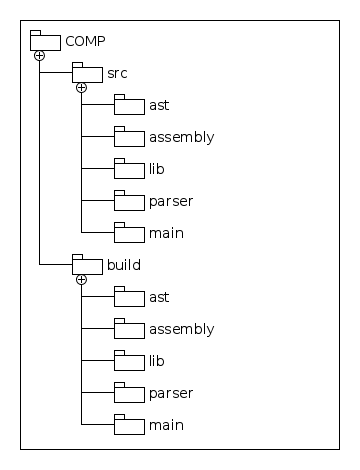
\includegraphics[height=8cm]{Folder_diagram}
\caption{Répartition des packages pour le compilateur}
\label{fig:Package}
\end{center}\end{figure}

\paragraph{Remarque :} le dossier build est similaire afin de conserver un stockage logique des .o lors de la compilation du projet.

\subsubsection{ast}
Le package ast contient l'ensemble des classes correspondant à ... l'ast ! Nous reviendrons plus en détail en partie \ref{subsec:Ast}.

\subsubsection{assembly}

Ce package contient l'ensemble des classes associées à la génération d'assembleur. En plus simple, c'est le dossier contenant le back-end.

\subsubsection{lib}

Il s'agit d'un petit dossier contenant le code unistd. Comme nous utilisons une fonction\footnote{getopt} de cette bibliothèque, ceux travaillant sur windows avaient besoin d'avoir ce fichier sous la main.

\subsubsection{parser}

C'est ici que se déroule le travail d'ANTLR4. Dans ce dossier se trouvent le fichier de grammaire, subtilement appelé \emph{expr.g4}, ainsi que l'ensemble des fichiers générés par ANTLR4. À cela s'ajoute notre première part de code : les visiteurs de symboles, situés dans les fichiers, tout aussi subtilement nommés, \emph{visiteur.cpp} et \emph{visiteur.hpp}.

\subsubsection{main}

Comme souvent, il est un peu seul, et il faut bien le mettre quelque part. Voilà l'endroit où se trouve \emph{main.cpp}. 

\subsection{Structure de l'ast}
\label{subsec:Ast}

Plutôt que de perdre du temps en mot, un diagramme de classe sera plus explicite (page \pageref{fig:BigAST}).
\begin{figure}[!hbt]\begin{center}
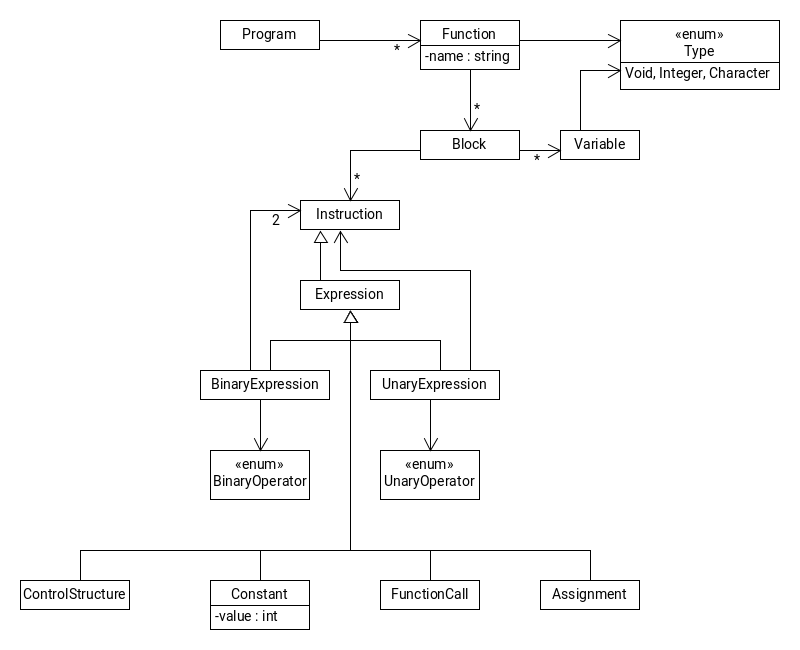
\includegraphics[width=\textwidth]{../ast_class_diagram.png}
\caption{Diagramme de classe complet de l'ast}
\label{fig:BigAST}
\end{center}\end{figure}

Si jamais ce diagramme semble indigeste à lire, en voici une version ne gardant que les liens d'héritage (page \pageref{fig:SmallAST})
\begin{sidewaysfigure}[!hbt]\begin{center}
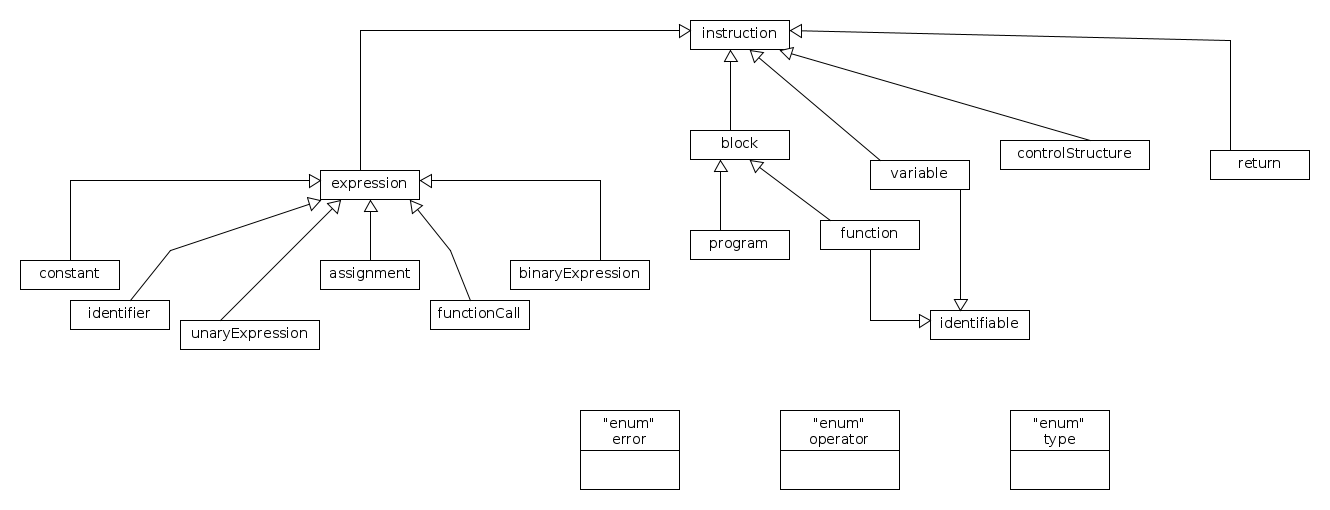
\includegraphics[width=\textwidth]{../diagramme_heritage.png} 
\caption{Diagramme de classe simplifié de l'ast}
\label{fig:SmallAST}
\end{center}\end{sidewaysfigure}

Pour bien comprendre ce diagramme, nous nous sommes fixés comme paradigme : \og tout est instruction \fg . Il reste ensuite quelques petits points à éclaircir, même si la plupart des éléments portent le même nom que ce soit à quoi il correspondent sémantiquement.\\
\paragraph{Variables, fonctions et identifiants} Les variables et les fonctions sont des éléments que l'on considère \emph{identifiables}. Ils portent un nom qui permet de bien les repérer. Cependant, voir le nom d'une variable n'a pas le même sens selon son contexte. Nous avons donc pris le parti suivant : définir/déclarer une variable revient à ajouter créer un objet \emph{Variable}, tout comme déclarer une fonction crée une \emph{Fonction}. En revanche, si l'on aperçoit le nom d'une variable/fonction en-dehors d'un contexte de déclaration, par exemple affectation ou appel de fonction, alors on crée un objet \emph{Identifier} qui signifie \og On fait appel à un truc donc on ne connait pas trop la nature \fg . Par exemple :\\

\begin{lstlisting}
int a, b=5; // a et b sont des Variables
a=b+3; // a et b sont des Identifier, 3 est une constant Integer.
\end{lstlisting}
\begin{lstlisting}
void main() {//main est une Fonction
}
main();// main est un Identifier
\end{lstlisting}
\section{Compiler le compilateur}
\label{sec:Compile}

\subsection{Compiler sur Linux}
\label{subsec:Linux}
Normalement, ça ne devrait pas être très compliqué. Il suffit de reprendre les variables localisant ANTLR4 dans le makefile et les adapter à votre installation d'ANTLR, similairement à l'exemple donné sur les machines de l'INSA.

\lstset{style=make}
\begin{lstlisting}
ANTLR=path/to/the/antlr4/executable
ANTLRSRC=path/to/the/antlr4/runtime/files
ANTLRRUNTIME=path/to/the/antlr4-runtime.a
\end{lstlisting}

En fonction de la manière dont vous définissez \bsc{ANTLRRUNTIME}, il faudra probablement aller modifier la définition de la variable \bsc{LDFLAGS}, un peu plus loin.\\
Il n'y aura ensuite plus qu'à se placer à la racine du projet, exécuter \emph{make} puis utiliser l'exécutable \textbf{./compiler}.

\subsection{Compiler sur Windows}
\label{subsec:Windows}

Il faut installer ANTLR4 adapter pour visual studio, puis lancer un projet visual studio en utilisant le code source fourni.\footnote{Pour être franc, nous n'avons pas vraiment unifié la manière de faire, chacun y allant de son mieux.}

\section{Gestion de projet}
\label{sec:Management}

Comme brillamment suggéré par le sujet, nous développons en mode AGILE. Comme pour toute méthode AGILE, nous adaptons le mot agile à notre sens. Cela prend la forme suivante : trois groupes de personnes travaillant chacun sur une partie de la chaîne de compilation.  Nous ajoutons à chaque itération de nouveaux éléments de grammaire, ensuite interprétés par les visiteurs, mis en forme dans l'ast et ensuite rédigé sous forme assembleur.
Voici les groupes :
\subsubsection{Officiellement}
\begin{itemize}
\item L. Ohl et I. Zemmouri : Grammaire, visiteurs, et comptes-rendus.
\item L. Saos : Responsable ast.
\item A. Belin, A. Nahid et A. Verrier : transcription de l'ast en assembleur.
\end{itemize}

Nous coordonnons régulièrement les parties afin de résoudre le plus vite les points pouvant être des goulots d'étranglement pour d'autres. Dans les faits, comprendre l'assembleur à pris beaucoup de temps, ce qui explique la grande avance prise par le frontend sur le backend.

\subsubsection{Officieusement}
\begin{itemize}
\item L. Ohl et I. Zemmouri : Grammaire, visiteurs, ragequit antlr et recherche de memes. Scribes lors des RTT.
\item L. Saos : Resposable ast, glorieux et officieux chef du bordel ambulant
\item A. Belin, A. Nahid et A. Verrier : pauvres victimes sacrifiées à l'assembleur
\end{itemize}

C'est le zbeul, mais dans la bonne humeur et le rire de voldemort !\footnote{He, hehe !}

\newpage
\section*{Annexe - Ce qui est en cours de route}
\label{sec:Annexe}
\subsection*{Grammaire}
La grammaire définit de nombreux points qui ne sont pas utilisés pour le moment, i.e. non visités. On y retrouve notamment : les includes, la définition de bloc de code, la construction du type char\footnote{Ce dernier est réellement visité toutefois}.
\subsection*{L'arithmétique}
Vous trouverez de par et d'autres, et notamment dans le fichier \emph{src/ast/operator.hpp} l'ensemble des opérateurs en cours de route. Sont actuellement en cours de développement : le \emph{ou}, le \emph{et}, le \emph{not} logiques.
\subsection*{L'ast}
L'ast possède de très nombreuses fonctionnalités encore non exploitées. À titre d'exemple, l'objet block, défini dans \emph{src/ast/block.hpp} permet de décrire un bloc de code de manière générale, et par extension une fonction. Il a été totalement écrit comme s'il devrait être utilisé similairement pur une boucle, une alternative, etc. À l'heure actuelle, il n'est employé que pour l'aspect \emph{fonction}.\\
D'autres objets sont également en cours de construction : \emph{functionCall}, \emph{ControlStructure}, etc.
\end{document}
